\section{Evaluating the Running Example}
\label{eval:example}

The security policy from the running example contains both static and dynamic elements,
and showcases all major features of the framework. It is therefore a good starting point
for evaluation. We have designed a number of testing scenarios based on it.

To quickly summarize, the security policy manages a building with workrooms, which are
statically assigned to projects, and lunchrooms, which are unassigned and limited by
capacity. At lunch time, workers can request seats in lunchrooms and the policy should
grant them access as soon as a seat becomes available, while upholding the overall
security goal: workers from different projects must not use the same room.

There are two main types of sub-ensembles in the policy. \cc{WorkroomAssignment} is
registered for each project and allows workers of the project to enter all workrooms
of that project. \cc{LunchroomAssignment} is registered for each lunchroom and ensures
that seats in that lunchroom are allocated as appropriate.

%%%

\subsection{Static Assignments}

The first scenario is in the morning, when workrooms are already open, but lunchrooms
are closed. Per the situation predicate, \cc{LunchroomAssignment}s are inactive, so only
statically-assigning \cc{WorkroomAssignment}s will be in play. Measuring their behavior
should give us a performance baseline.

There are 100 workrooms that are assigned in a round-robin fashion to the configured
number of projects. We have set up three test cases, for 5, 15, and 50 projects. In each
case, we vary the number of workers from 500 to 10~000 in increments of 500. Each
configuration is tested 500 times.

\begin{figure}[ht]
    \centering
    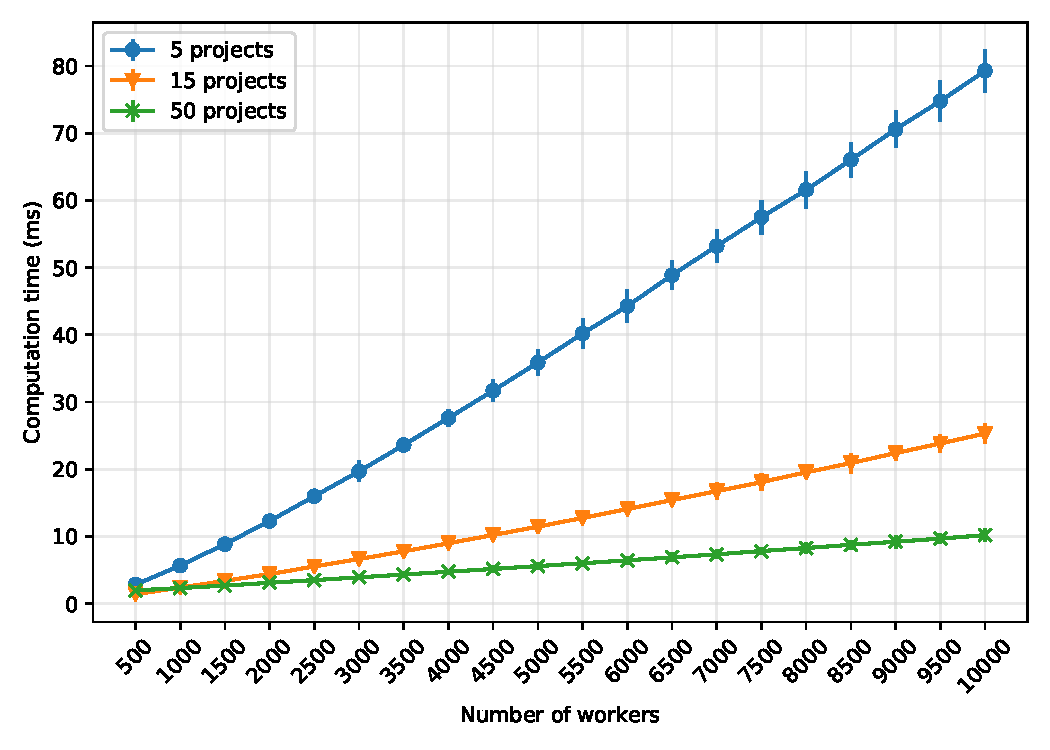
\includegraphics[width=1\linewidth]{img/workers-simple.pdf}
    \caption{Static assignment to workrooms}
    \label{fig:workers-simple}
\end{figure}

Figure~\ref{fig:workers-simple} shows the results of measurements. Vertical lines from
the points represent error bars of one standard deviation; in many cases, too small to
be visible over the point marker.

Computation time grows linearly with the total number of access grants. For this reason,
times for the 5-project test case are larger: the number of workrooms is fixed, so each
project gets more rooms and each worker gets an access grant to each of the rooms.

The measurements are in the millisecond range, and it is possible to process 10~000
workers in 80~ms. Most of the time is actually spent pre-generating a lookup table for
the \cc{allows()} method; when this feature is disabled, computation times drop as much
as 4x for the largest configuration.

%%%

\subsection{Empty Lunchrooms}
\label{eval:example:dynamic}

At lunch time, \cc{LunchroomAssignment} ensembles are activated, and workers can request
seats by setting their \cc{hungry} attribute to true. In the second scenario, we assume
that all available lunchrooms are empty, and the solver is attempting to seat an
increasing number of hungry workers.

From the outset, it is clear that the problem has an exponentially large solution space.
The solver is attempting to maximize a utility expression: $\sum |s_i|^2$, where $s_i$
is the set of occupied seats in $i$-th lunchroom. Even with the knowledge that only the
cardinality of seatings matters, the search still needs to implicitly consider all
possible assignments of projects to lunchrooms, and all possible distributions of
workers between the available rooms.

\begin{figure}[ht]
    \centering
    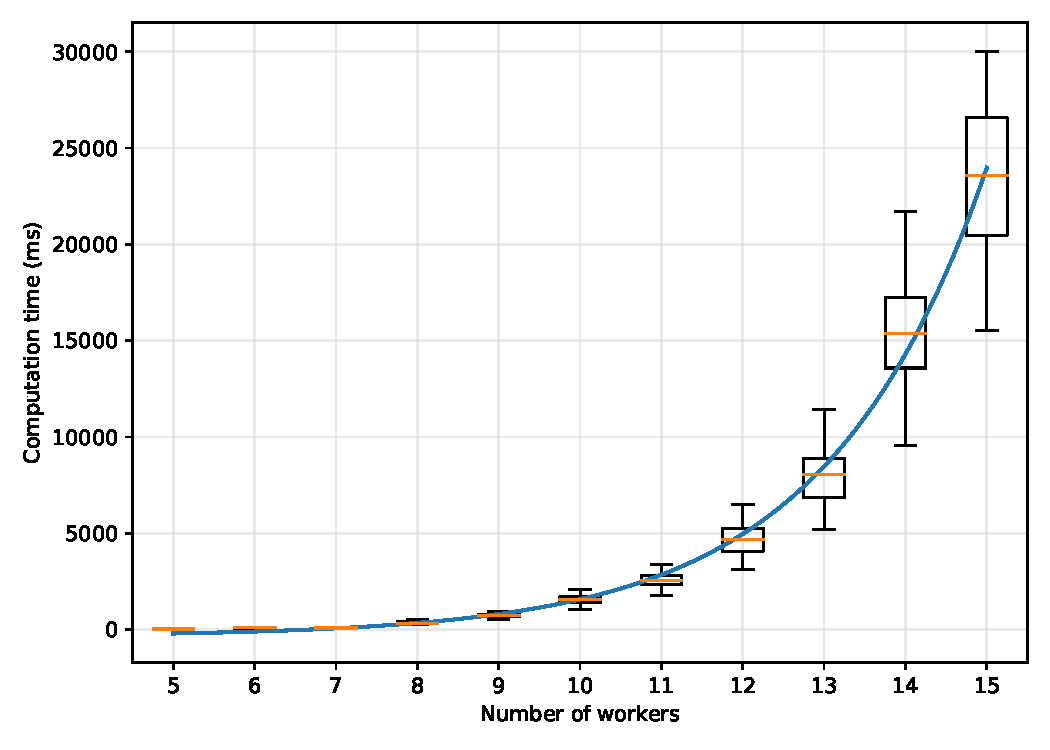
\includegraphics[width=1\linewidth]{img/workers-morerooms.pdf}
    \caption{Dynamic assignment with more rooms than projects}
    \label{fig:workers-morerooms}
\end{figure}

The test case in figure~\ref{fig:workers-morerooms} has 4 lunchrooms with 10 seats
each, and 3 available projects. Individual configurations then specify a total number
of hungry workers, which are selected from the projects in a round-robin fashion.

The Y axis represents time to find an optimal solution. Each configuration is rendered
as a box plot over the test runs, with whiskers representing 1.5 IQR, and outliers
removed. The blue line is an exponential curve fitted to the medians.

Even in this very small test case, computation times are unacceptably slow. Seating 12
workers takes 5 seconds, and the solver crosses the 30 second time limit at the 16
worker mark\footnote{The solver was able to find the optimal solution under 30 seconds
in several cases, but it timed out in most of the 100 test runs. For this reason, we
have excluded this data entirely.}.

\medskip

The situation with more available lunchrooms than projects represents the worst case for
the solver: it is certain that at least one project will be able to use more than one
room, so workers from that project can be distributed among the available rooms.

This factor is removed in the next scenario. Number of lunchrooms is fixed to 3, each
with 5 seats, and number of projects varies from 5 to 9. Same as in previous scenario,
the lunchrooms are empty and we are seating an increasing number of hungry workers.

\begin{figure}[ht]
    \centering
    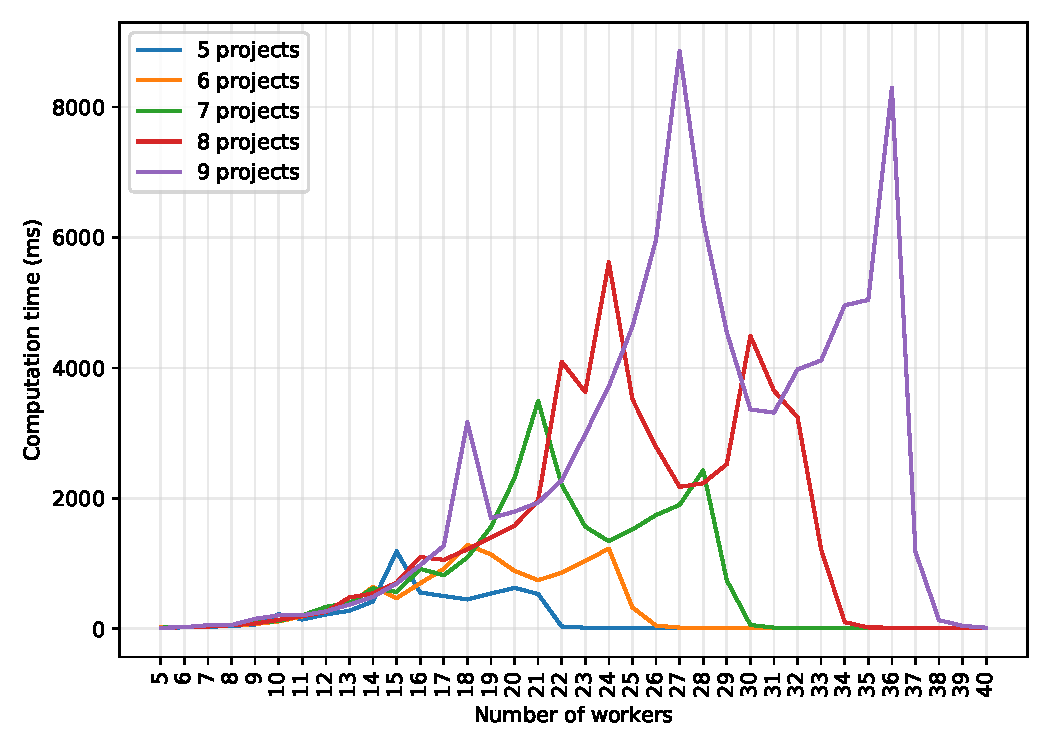
\includegraphics[width=1\linewidth]{img/workers-moreprojects.pdf}
    \caption{Dynamic assignment with more projects than rooms}
    \label{fig:workers-moreprojects}
\end{figure}

The search is simplified by the fact that in terms of utility, distributing workers from
the same project across rooms is always worse than putting them together and using
workers from a different project for the other rooms. Although the number of solutions
is still exponential, computation times are much lower.

Figure~\ref{fig:workers-moreprojects} shows the results. Variance in computation times
is comparable to the previous scenario, so we are only showing median times to optimal
solution. Two outlier configurations have been omitted: 6 projects with 35 workers, and
8 projects with 39 workers. See section~\ref{eval:example:badsolver} for discussion.
After that, the longest time recorded is approx. 9 seconds, for 27 workers in 9
projects.

An interesting property is visible here. The peak times correspond to multiples of the
number of projects, and after $4p + 1$ workers, computation times sharply drop to
\textasciitilde{}10~ms. This point corresponds to the moment when the round-robin
algorithm first picks 5 hungry workers (same as lunchroom capacity) from the same
project. As soon as a lunchroom can be filled to capacity by a single project, the
solver seems to be able to use this fact to optimize the search.

Similarly, multiples of number of projects are the points when the same number of
workers is picked from every project. At that point, all projects are equally good
candidates for seating, and so the number of solutions rises; after the peak, it is
possible to quickly exclude the projects with fewer hungry workers.

Although the computation is still relatively slow, we are now within realistic problem
sizes. In a real-world deployment, seating 30 workers in 5 seconds might be acceptable.

%%%

\subsection{Probabilistic Search Anomalies}
\label{eval:example:badsolver}

In the previous scenario, we observed that when a trivial solution of a certain type
exists, the solver converges on that solution very quickly. In particular, when it is
possible to fill a room to capacity, an optimal solution is found in milliseconds. This
result was stable across runs and not affected by the number of ``overflow'' workers who
are hungry but could not be seated.

However, in some cases, the optimization seems to fail. This often appears in the form
of outliers --- in a particular configuration, most attempts take 20~ms, but some can
take several seconds. For some configurations, the short times are actually the
outliers: most attempts take several seconds, and the occasional ``good try'' completes
immediately.

We have not found a pattern in the bad configurations. The outliers in good
configurations behave probabilistically and appear more frequently as configuration size
grows.

To measure this behavior, we have set up the following scenario: the number of projects
is the same as the number of lunchrooms, each lunchroom has a capacity of 5, and there
are 5 hungry workers per project. The trivial solution is apparent: each lunchroom
is filled to capacity with workers from one project, and the remaining search space
is only as big as the number of project-lunchroom permutations.

\begin{figure}[ht]
    \centering
    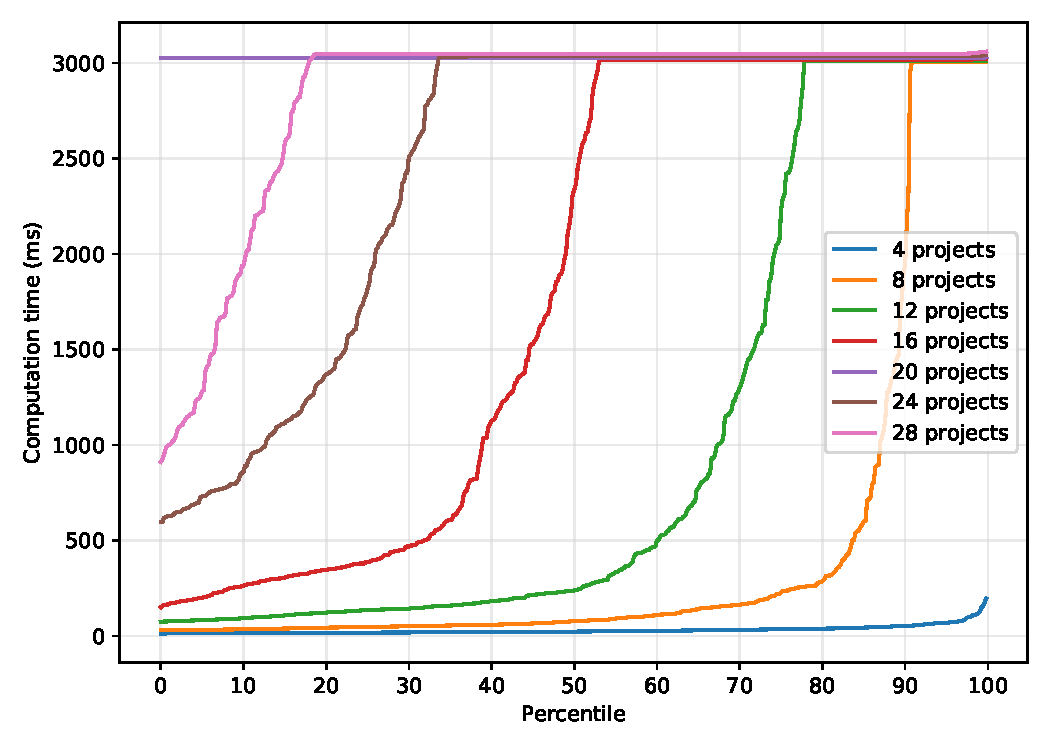
\includegraphics[width=1\linewidth]{img/badsolver.pdf}
    \caption{Frequency of search anomalies}
    \label{fig:badsolver}
\end{figure}

We created configurations of 1 to 30 projects, and ran 500 tests of each, with a time
limit of 3 seconds. The expected solving time of one run is below 100~ms, so this time
limit was deemed sufficient. Results are shown as a percentile graph in
figure~\ref{fig:badsolver}. We arbitrarily chose to plot multiples of 4. Showing more
configurations does not bring any additional insights and makes the graph less clear.

For 4 projects, all tests finished under 500~ms. At 12 projects, 60~\% of tests finished
under 500~ms, and 25~\% of tests timed out. 28 projects is large enough that no test
finished under 500~ms, but the curve still has a similar shape; presumably, the
likelihood of finding the good solution is too low.

The configuration with 20 projects is a ``bad'' one, as all of the 500 attempts have
timed out.

%%%

\subsection{Solver Time Limits}
\label{eval:example:limits}

In all previous scenarios, we measured time to find an \textit{optimal} solution. When
the search timed out before declaring a solution optimal, it was counted as a failure.
However, that does not mean that \textit{no} solutions were found.

Choco's optimization process works by finding a satisfying solution for the problem and
then posting an additional constraint that the next solution must have a strictly higher
utility. Most of the time this means iterating over several successively better
solutions. If an optimal solution is not required, it is possible to either switch the
behavior of the solver, or to accept the best solution found when the time limit is
reached.

To test the trade-off between speed and solution quality, a scenario was set up with 3
projects, 5 lunchrooms with 20 seats each, and 21 hungry workers, 7 per project. In
this scenario, the optimal solution is seating all of the workers from a single project
in one of the available lunchrooms, and keeping two rooms empty. The total utility
of this solution is $7^2 \cdot 3 + 0 \cdot 2 = 147$.

\begin{figure}[ht]
    \centering
    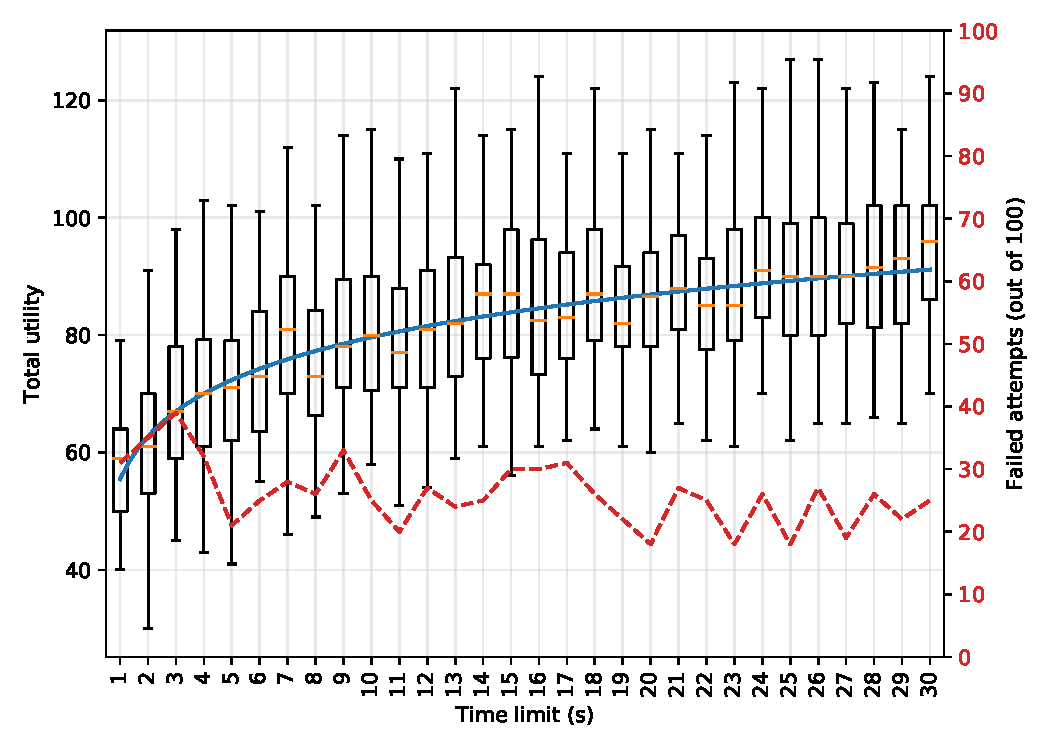
\includegraphics[width=1\linewidth]{img/timelimits.pdf}
    \caption{Utility of solutions found before time limit}
    \label{fig:timelimits}
\end{figure}

We created configurations with a successively higher time limit from 1 to 30 seconds,
and measured them over 100 runs. Figure~\ref{fig:timelimits} shows each configuration as
a box plot over successful tests, with whiskers representing 1.5 IQR, and outliers
removed. A relatively large amount of tests have failed to find a solution within the
time limit. The red dashed line shows the amount for each configuration. Over 50
attempts were successful in every case, which gives us a sufficient number of samples.

The data has high variance, but the successful runs copy a logarithmic curve (shown in
blue). That is the expected behavior. On an exponential problem, linear increase in
computation time should provide logarithmic benefits.

None of the test runs get close to the optimal utility of 147. In preliminary
experiments, even tests with a time limit of 5 minutes did not converge on the optimal
solution. These results also retroactively show that our choice of 30 seconds as the
default time limit was reasonable.

%%%

\subsection{Practical Situations}
\label{eval:example:practical}

Previous scenarios were testing the solver on arbitrary configurations in isolation. In
a real-world deployment, however, the situation would look very different.

First thing to note is that in practice, it is almost impossible for dozens of workers
to request lunch at exactly the same time. We have experimented with a ``one-by-one''
solving method, where instead of submitting all hungry workers to the solver at once, we
incrementally submit one worker at a time. This converts the $O(k^N)$ problem of seating
$N$ workers to $N$ separate $O(1)$ problems of seating one worker. In most cases, this
approach will achieve the same utility, because workers from the same project are
preferentially seated together. Computation time grows linearly with the number of
workers.

\begin{figure}[ht]
    \centering
    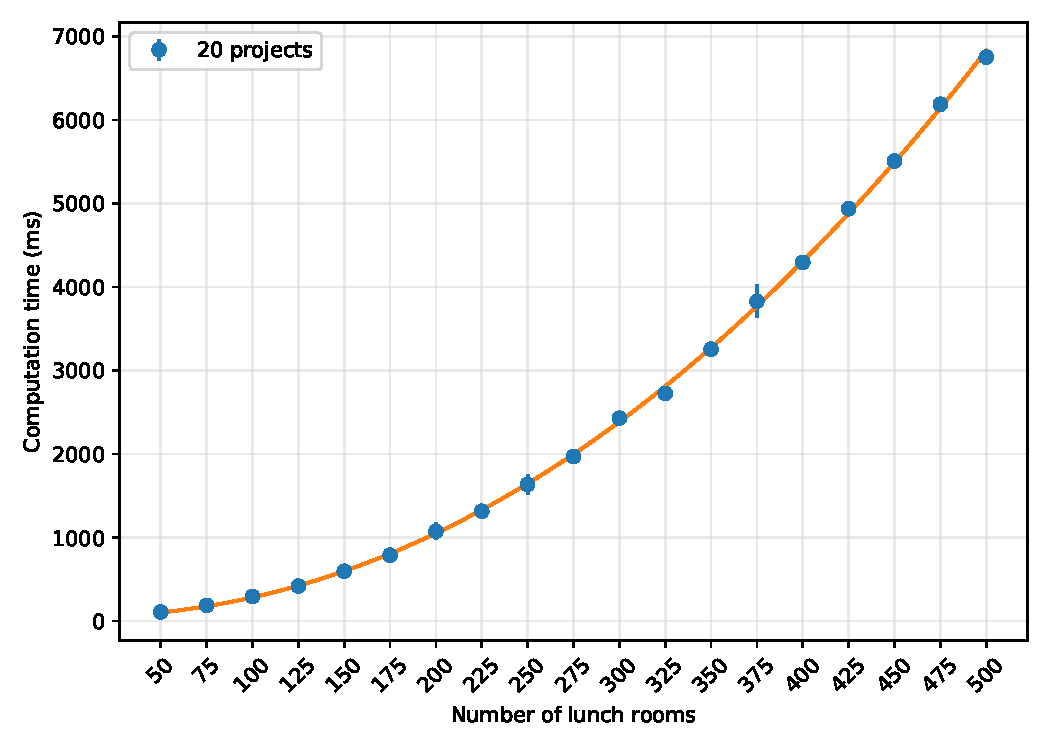
\includegraphics[width=1\linewidth]{img/workers-oneworker.pdf}
    \caption{Time to seating one worker}
    \label{fig:workers-oneworker}
\end{figure}

Figure~\ref{fig:workers-oneworker} shows computation times for seating one worker in an
increasing number of lunchrooms. Each case was measured 100 times. Blue dots represent
median times, vertical lines are error bars of one standard deviation.

The number of projects is irrelevant, as the worker being seated can only belong to one,
and lunchrooms are only tied to projects through their occupants. Lunchroom capacity is
also irrelevant, as long as it is 1 or more. At 200 lunchrooms, one worker can be seated
in one second, which is probably good enough for any reasonable real-world deployment.

Solving time is perfectly quadratic (shown in orange) in the number of lunchrooms. The
source of the quadratic behavior is most likely the \cc{allDisjoint} constraint: a
worker can be seated in any of the $N$ rooms, and for each variant, $N$ rooms must be
checked to ensure disjointness.

%%%

\subsection{Simulation}
\label{eval:example:simulation}

In practical situations, it is also very rare for all lunchrooms to be empty at the
same time. When the first worker is seated in a lunchroom, the choice locks the
worker's project to that room. All subsequent requesters from the same project will be
preferentially seated there. This effectively splits the problem in two: workers from a
chosen project will only be seated to that project's rooms, while these are excluded
from the possibilities for workers of other projects.

In order to examine this behavior, and to test the solver in more real-world-like
conditions, we have created a simulation of worker behavior at lunch time. The basis of
the simulation is a building with 500 workers working on 10 projects, which is realistic
for a modern office building. On each of the 5 floors there is a lunchroom with 40
seats.

At every step of the simulation, every worker that hasn't eaten yet has a 0,5~\% chance
of becoming hungry and requesting a seat. Once a worker receives a seating notification,
they take up to 5 simulation steps to reach the lunchroom, and then 5 to 20 steps to
eat, before leaving the lunchroom and getting back to work.

In a typical simulation run, all workers can have lunch in about 2~000 steps. We are not
particularly interested in the tail end of the simulation, because it mostly involves
waiting for workers to finish eating. Therefore, we stop the simulation after 1~500
steps, and run the first 1~500 steps 100 times, for a total of 150~000 steps.

\begin{figure}[ht]
    \centering
    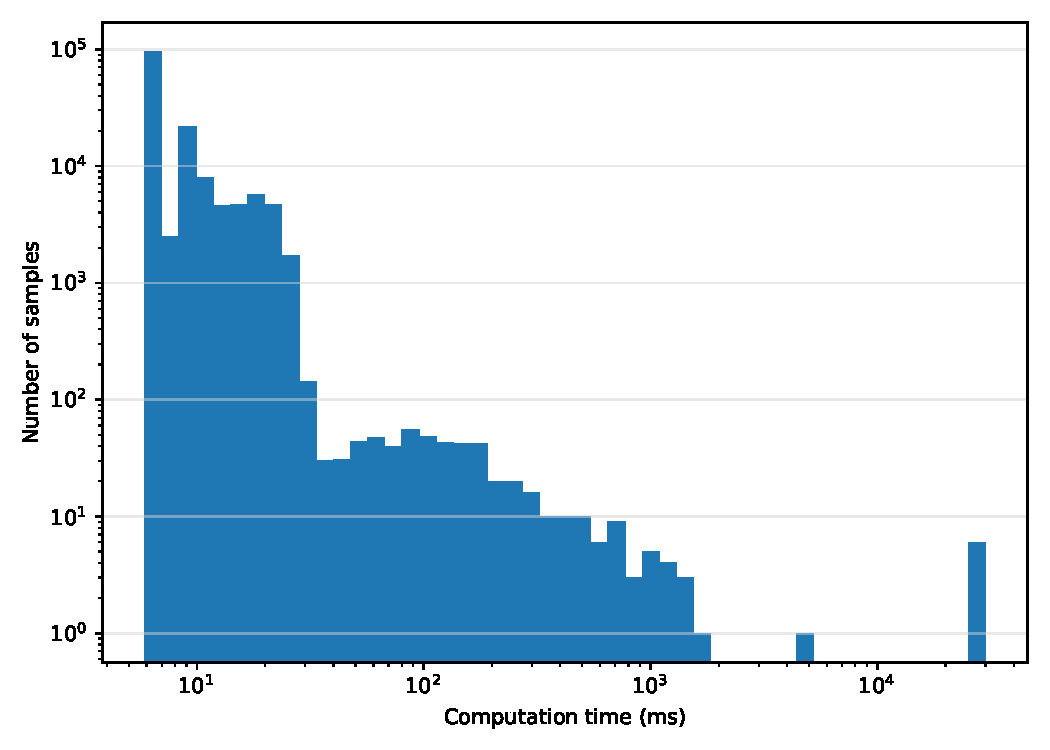
\includegraphics[width=1\linewidth]{img/simulation.pdf}
    \caption{Histogram of computation times per simulation step}
    \label{fig:simulation}
\end{figure}

Figure~\ref{fig:simulation} is a histogram of computation times per one simulation step,
with both axes logarithmic. The median step time is 6.4~ms, and mean step time is
10.7~ms. Out of the 150~000 measurements, only 285 took more than 100~ms.

There is a small number of outliers that do not find the optimal solution within the 30
second time limit. However, an important feature of this kind of setup is that it can
recover very fast from such failure. In the rare case where a difficult configuration
arises, such as when two lunchrooms become available in the same simulation step, a
sub-optimal seating solution will still place some workers in at least one of the rooms.
Subsequent solver runs can continue off this result and place the remaining workers. We
have never observed more than one failure in a row.

From these results, we conclude that the performance of the framework is suitable for
real-world deployment.
